% ============================================================
%  Sentence Memorability Study — Beamer Presentation
%  Compile with: pdflatex slides.tex  (run twice for ToC)
% ============================================================
\documentclass[aspectratio=169, 10pt]{beamer}

% ── Theme ────────────────────────────────────────────────────
\usetheme{Madrid}
\usecolortheme{default}
\usefonttheme{professionalfonts}
\setbeamertemplate{navigation symbols}{}
\setbeamertemplate{footline}[frame number]
% ── Green structure colour ────────────────────────────────────
\setbeamercolor{structure}{fg=green!45!black}
\setbeamercolor{palette primary}{bg=green!45!black, fg=white}
\setbeamercolor{palette secondary}{bg=green!35!black, fg=white}
\setbeamercolor{palette tertiary}{bg=green!25!black, fg=white}
\setbeamercolor{palette quaternary}{bg=green!20!black, fg=white}
\setbeamercolor{titlelike}{parent=palette primary}
\setbeamercolor{frametitle}{bg=green!40!black, fg=white}
% ── Block colours ────────────────────────────────────────────
\setbeamercolor{block title}{bg=green!20!white, fg=green!30!black}
\setbeamercolor{block body}{bg=green!5!white}
\setbeamercolor{alertblock title}{bg=red!20!white, fg=red!40!black}
\setbeamercolor{alertblock body}{bg=red!5!white}
\setbeamercolor{exampleblock title}{bg=green!35!white, fg=green!40!black}
\setbeamercolor{exampleblock body}{bg=green!10!white}

% ── Packages ─────────────────────────────────────────────────
\usepackage{graphicx}
\usepackage{booktabs}
\usepackage{array}
\usepackage{multirow}
\usepackage{xcolor}
\usepackage{amsmath}
\usepackage{siunitx}

% ── Convenience macros ───────────────────────────────────────
\newcommand{\pval}[1]{\textit{p}\,=\,#1}
\newcommand{\sig}[1]{\textcolor{red!70!black}{\textbf{#1}}}
\newcommand{\ns}[1]{\textcolor{gray}{#1}}
\newcommand{\kw}[3]{$\chi^{2}(#1)=#2$, \pval{#3}}  % KW shorthand

% ── Meta ─────────────────────────────────────────────────────
\title[Sentence Memorability]{%
  \textbf{Does Noun Imageability Affect Sentence Memorability?}\\[4pt]
  \normalsize A Non-Parametric Analysis of Immediate and Wording Recognition}
\subtitle{Continuous Recognition Memory Paradigm}
\author{Team: Idle Death Gamblers}
\institute{Semester 6 Research Methods}
\date{March 2026}

% ============================================================
\begin{document}

% ── Title frame ──────────────────────────────────────────────
\begin{frame}
  \titlepage
\end{frame}

% ── Outline ──────────────────────────────────────────────────
\begin{frame}{Outline}
  \tableofcontents[hideallsubsections]
\end{frame}

% ============================================================
\section{Background \& Research Question}
% ============================================================

\begin{frame}{Theoretical Background}
  \begin{itemize}
    \item \textbf{Meaning vs. Wording:} The meaning of a concrete sentence is represented in memory as a nonverbal spatial image, whereas individual words are stored as sequential verbal strings. Meaning judgments decrease in accuracy over time, but wording judgments are independent of meaning memory.
    \item \textbf{Reconstructive Process:} Sentence recall is a constructive activity. Listeners extract a semantic representation and later reconstruct the surface structure based on salient themes and an inherent preference for active constructions.
    \item \textbf{Syntactic Storage:} Syntactic features are not stored as single, independent elements in a memory trace. Instead, syntactic form is often reconstructed from other semantic memories at the time of retrieval.
  \end{itemize}
\end{frame}

\begin{frame}{Motivation}
  \begin{columns}[T]
    \column{0.55\textwidth}
      \begin{block}{Core Question}
        Does the \textbf{imageability} of the main noun in a sentence
        affect how well participants \emph{recognise} the sentence
        later — and how accurately they remember its exact wording? 
      \end{block}
      \vspace{0.5em}
      \textbf{Why it matters:}
      \begin{itemize}
        \item Imageability (ease of forming a mental image) is a
              known predictor of word-level recall.
        \item Less is known about its role at the \emph{sentence}
              level, and whether the \emph{voice} (active vs passive)
              of a target sentence modulates that effect.
      \end{itemize}

    \column{0.42\textwidth}
      \begin{block}{Noun Imageability Conditions}
        \begin{tabular}{lll}
          \toprule
          Code & Subject & Object \\
          \midrule
          \textbf{HH} & High & High \\
          \textbf{HL} & High & Low  \\
          \textbf{LH} & Low  & High \\
          \textbf{LL} & Low  & Low  \\
          \bottomrule
        \end{tabular}\\[4pt]
        \small HF fillers used for signal-detection FA baseline.
      \end{block}
  \end{columns}
\end{frame}

\begin{frame}{Hypotheses}
  \begin{enumerate}
    \item[\textbf{H1}] Sentences with higher noun imageability will
          yield higher \textbf{Immediate Recognition (IR)} corrected
          scores (CR$_\text{IR}$).
    \vspace{0.5em}
    \item[\textbf{H2}] Imageability will also facilitate
          \textbf{Wording Recognition (WR)}, reflected in higher
          conditional WR accuracy.
    \vspace{0.5em}
    \item[\textbf{H3}] Participants will be faster to respond (shorter
          RT) to high-imageability sentences.
    \vspace{0.5em}
    \item[\textbf{H4}] \textbf{Voice} (active vs passive) will interact
          with imageability — passive constructions may reduce the
          imageability benefit.
  \end{enumerate}
\end{frame}

% ============================================================
\section{Experimental Design}
% ============================================================

\begin{frame}{Continuous Recognition Memory Paradigm}
  \begin{columns}[T]
    \column{0.48\textwidth}
      \textbf{Structure}
      \begin{itemize}
        \item 3 experimental \emph{blocks} per participant.
        \item Each block: study phase + probe phase.
        \item \textbf{48 target sentences} per participant
              (4 conditions $\times$ 2 voices $\times$ 6 sentences).
        \item Sample Goal: Power analysis indicated 334 participants were required for our hypotheses.
      \end{itemize}
      \vspace{0.5em}
      \textbf{Responses}
      \begin{itemize}
        \item \textbf{IR key}: ``I recognise this sentence''
        \item \textbf{WR key}: ``I recognise the exact wording''
      \end{itemize}

    \column{0.48\textwidth}
      \textbf{Signal-Detection Scoring}
      \begin{block}{Immediate Recognition}
        $\text{CR}_\text{IR} = \text{Hit Rate} - \text{FA Rate}$\\[4pt]
        \small
        Hit = IR pressed on target probe\\
        FA  = IR pressed on HF first-showing 
      \end{block}
      \begin{block}{Wording Recognition}
        $\text{Acc}_\text{WR} = \dfrac{n(\text{wr\_accuracy}=1)}{n(\text{WR trials})}$
        \vspace{2pt}
        \small Conditional: only participants who pressed WR;\\
        wr\_accuracy = 1 iff same-voice probe recognised 
      \end{block}
  \end{columns}
\end{frame}

% ============================================================
\section{Data Pipeline \& Validation}
% ============================================================

\begin{frame}{Participant Validation}
  \begin{columns}[T]
    \column{0.50\textwidth}
      \textbf{Validation Formula (per block)}
      \[
        \text{Correct} > \frac{\text{Wrong}}{2} + \text{Missed}
      \]
      \vspace{0.3em}
      Applied to each of the 3 blocks per participant. A block \emph{fails} if the inequality is not satisfied.

      \vspace{0.5em}
      \textbf{Exclusion policy:} data from failed blocks is dropped; a participant is \emph{retained} as long as they have \textbf{at least one valid block}. Only participants who fail \emph{all} blocks are excluded.

    \column{0.46\textwidth}
      \begin{block}{Block-Level Pass/Fail}
        \begin{tabular}{ccc}
          \toprule
          Block & Failed & Passed \\
          \midrule
          1 & 6  & 108 \\
          2 & 5  & 109 \\
          3 & 2  & 112 \\
          \bottomrule
        \end{tabular}
      \end{block}
      \begin{exampleblock}{Final Sample}
        \begin{tabular}{ll}
          Total enrolled   & 114 \\
          \textbf{Retained} & \textbf{112 (98.2\%)} \\
          Excluded (0 valid blocks) & 2 (1.8\%)  \\
        \end{tabular}
      \end{exampleblock}
  \end{columns}
\end{frame}

\begin{frame}{RT Outlier Trimming}
  \begin{block}{Criterion (per participant, per RT type)}
    Replace with \texttt{NA} if: $\text{RT} < 200\,\text{ms}$
    \quad or \quad $\text{RT} > \bar{x}_\text{participant} + 3\,\text{SD}$ 
  \end{block}
  \vspace{0.8em}
  \begin{center}
    \begin{tabular}{lrr}
      \toprule
      Measure & Values trimmed & \% of valid RTs \\
      \midrule
      IR Reaction Time & 177  & $<0.4\%$ \\
      WR Reaction Time & 1{,}239 & $\approx2.5\%$  \\
      \bottomrule
    \end{tabular}
  \end{center}
  \vspace{0.5em}
  \small Accuracy data is \emph{preserved}; only the RT value is set to NA.
  WR trimming is higher because WR RTs include cross-voice probes
  which are intrinsically slower.
\end{frame}

% ============================================================
\section{Descriptive Statistics}
% ============================================================

\begin{frame}{False Alarm Rates — IR}
  \begin{columns}[T]
    \column{0.50\textwidth}
      \textbf{Computation}\\[4pt]
      \small Denominator: HF filler \emph{first-showings}
      (is\_probe\_repeat $= \text{NA}$).\\
      Numerator: IR key pressed on those first-showings.\\[6pt]
      \[
        \text{FA Rate}_\text{IR} =
          \frac{n(\text{IR pressed on HF first-showing})}
               {n(\text{HF first-showings shown})}
      \]

    \column{0.46\textwidth}
      \begin{block}{Participant-Level FA Rate Summary}
        \begin{tabular}{lr}
          \toprule
          Statistic & Value \\
          \midrule
          Mean  & 0.160 \\
          SD    & 0.104 \\
          Min   & 0.000 \\
          Max   & 0.427 \\
          \midrule
          HF first-showings / participant & 64–96 \\
          \bottomrule
        \end{tabular}
      \end{block}
  \end{columns}
  \vspace{0.4em}
  \small Substantial individual variability in FA rate confirms
  signal-detection correction is critical.
\end{frame}

\begin{frame}{IR Corrected Recognition — Descriptives}
  \renewcommand{\arraystretch}{1.15}
  \begin{center}
  \small
  \begin{tabular}{lllrrrrr}
    \toprule
    \textbf{Cond.} & \textbf{Voice} & $N$ & \textbf{Mean} & \textbf{Median} & \textbf{IQR} & \textbf{Skew} & \textbf{Kurt.} \\
    \midrule
    HH & Active  & 112 & 0.683 & 0.729 & 0.273 & $-0.79$ & 3.52 \\
    HH & Passive & 112 & 0.695 & 0.750 & 0.281 & $-1.29$ & 5.03 \\
    \addlinespace
    HL & Active  & 112 & 0.689 & 0.734 & 0.281 & $-0.78$ & 3.22 \\
    HL & Passive & 112 & 0.693 & 0.740 & 0.291 & $-0.98$ & 3.88 \\
    \addlinespace
    LH & Active  & 112 & 0.677 & 0.703 & 0.250 & $-0.79$ & 3.74 \\
    LH & Passive & 112 & 0.681 & 0.740 & 0.294 & $-1.04$ & 3.86 \\
    \addlinespace
    \sig{LL} & \sig{Active}  & \sig{112} & \sig{0.625} & \sig{0.641} & \sig{0.273} & \sig{$-0.48$} & \sig{2.65} \\
    \sig{LL} & \sig{Passive} & \sig{112} & \sig{0.638} & \sig{0.635} & \sig{0.255} & \sig{$-0.47$} & \sig{2.64}  \\
    \bottomrule
  \end{tabular}
  \end{center}
  \vspace{0.3em}
  \small \sig{Red = LL condition} that shows consistently lower CR scores.
  All conditions display negative skew, indicating ceiling-like performance.
\end{frame}

\begin{frame}{WR Conditional Accuracy — Descriptives}
  \renewcommand{\arraystretch}{1.15}
  \begin{center}
  \small
  \begin{tabular}{lllrrrrr}
    \toprule
    \textbf{Cond.} & \textbf{Voice} & $N$ & \textbf{Mean} & \textbf{Median} & \textbf{IQR} & \textbf{Skew} & \textbf{Kurt.} \\
    \midrule
    HH & Active  & 112 & 0.742 & 0.750 & 0.275 & $-0.46$ & 3.30 \\
    HH & Passive & 111 & 0.752 & 0.800 & 0.367 & $-0.50$ & 2.32 \\
    \addlinespace
    HL & Active  & 112 & 0.775 & 0.817 & 0.333 & $-1.23$ & 5.10 \\
    HL & Passive & 111 & 0.720 & 0.750 & 0.292 & $-0.98$ & 3.98 \\
    \addlinespace
    LH & Active  & 111 & 0.769 & 0.800 & 0.333 & $-0.49$ & 2.27 \\
    LH & Passive & 111 & 0.755 & 0.800 & 0.250 & $-1.04$ & 4.55 \\
    \addlinespace
    LL & Active  & 110 & 0.744 & 0.750 & 0.233 & $-0.83$ & 3.44 \\
    LL & Passive & 112 & 0.717 & 0.750 & 0.233 & $-0.83$ & 3.44  \\
    \bottomrule
  \end{tabular}
  \end{center}
  \vspace{0.3em}
  \small WR accuracy is uniformly high ($\approx 0.72$–$0.78$) and does not
  show the same LL dip as IR CR; negative skew throughout.
  Mean global IR-WR distance $\approx 0.07$--$0.09$ per condition.
\end{frame}

% ============================================================
\section{Normality \& Test Selection}
% ============================================================

\begin{frame}{Normality Tests — Shapiro-Wilk}
  \begin{block}{Hypotheses}
    $H_0$: sample drawn from a normal distribution.
    Rejection (\pval{< .05}) \textbf{justifies non-parametric tests}.
  \end{block}
  \vspace{0.6em}
  \begin{center}
  \renewcommand{\arraystretch}{1.2}
  \begin{tabular}{lrrl}
    \toprule
    \textbf{Metric} & $n$ & $W$ & \pval{} \\
    \midrule
    IR Corrected Recognition    & 896 & 0.9406 & $1.86 \times 10^{-18}$ \\
    IR Reaction Time            & 890 & 0.9836 & $1.98 \times 10^{-8}$  \\
    WR Accuracy Score           & 890 & 0.9112 & $2.25 \times 10^{-22}$ \\
    WR Reaction Time            & 877 & 0.8658 & $9.94 \times 10^{-27}$  \\
    \bottomrule
  \end{tabular}
  \end{center}
  \vspace{0.5em}
  \begin{alertblock}{Conclusion}
    \textbf{All four metrics are severely non-normal} ($p \ll .001$).
    Parametric ANOVA is \emph{not} appropriate.\\
    \textbf{Selected tests:} Kruskal-Wallis (omnibus)
    $\to$ Pairwise Wilcoxon (post-hoc)
    $\to$ Scheirer-Ray-Hare (2-way interaction).
  \end{alertblock}
\end{frame}

% ============================================================
\section{Results — Inferential Statistics}
% ============================================================

\begin{frame}{Raincloud Plot — IR Corrected Recognition}
  \begin{center}
    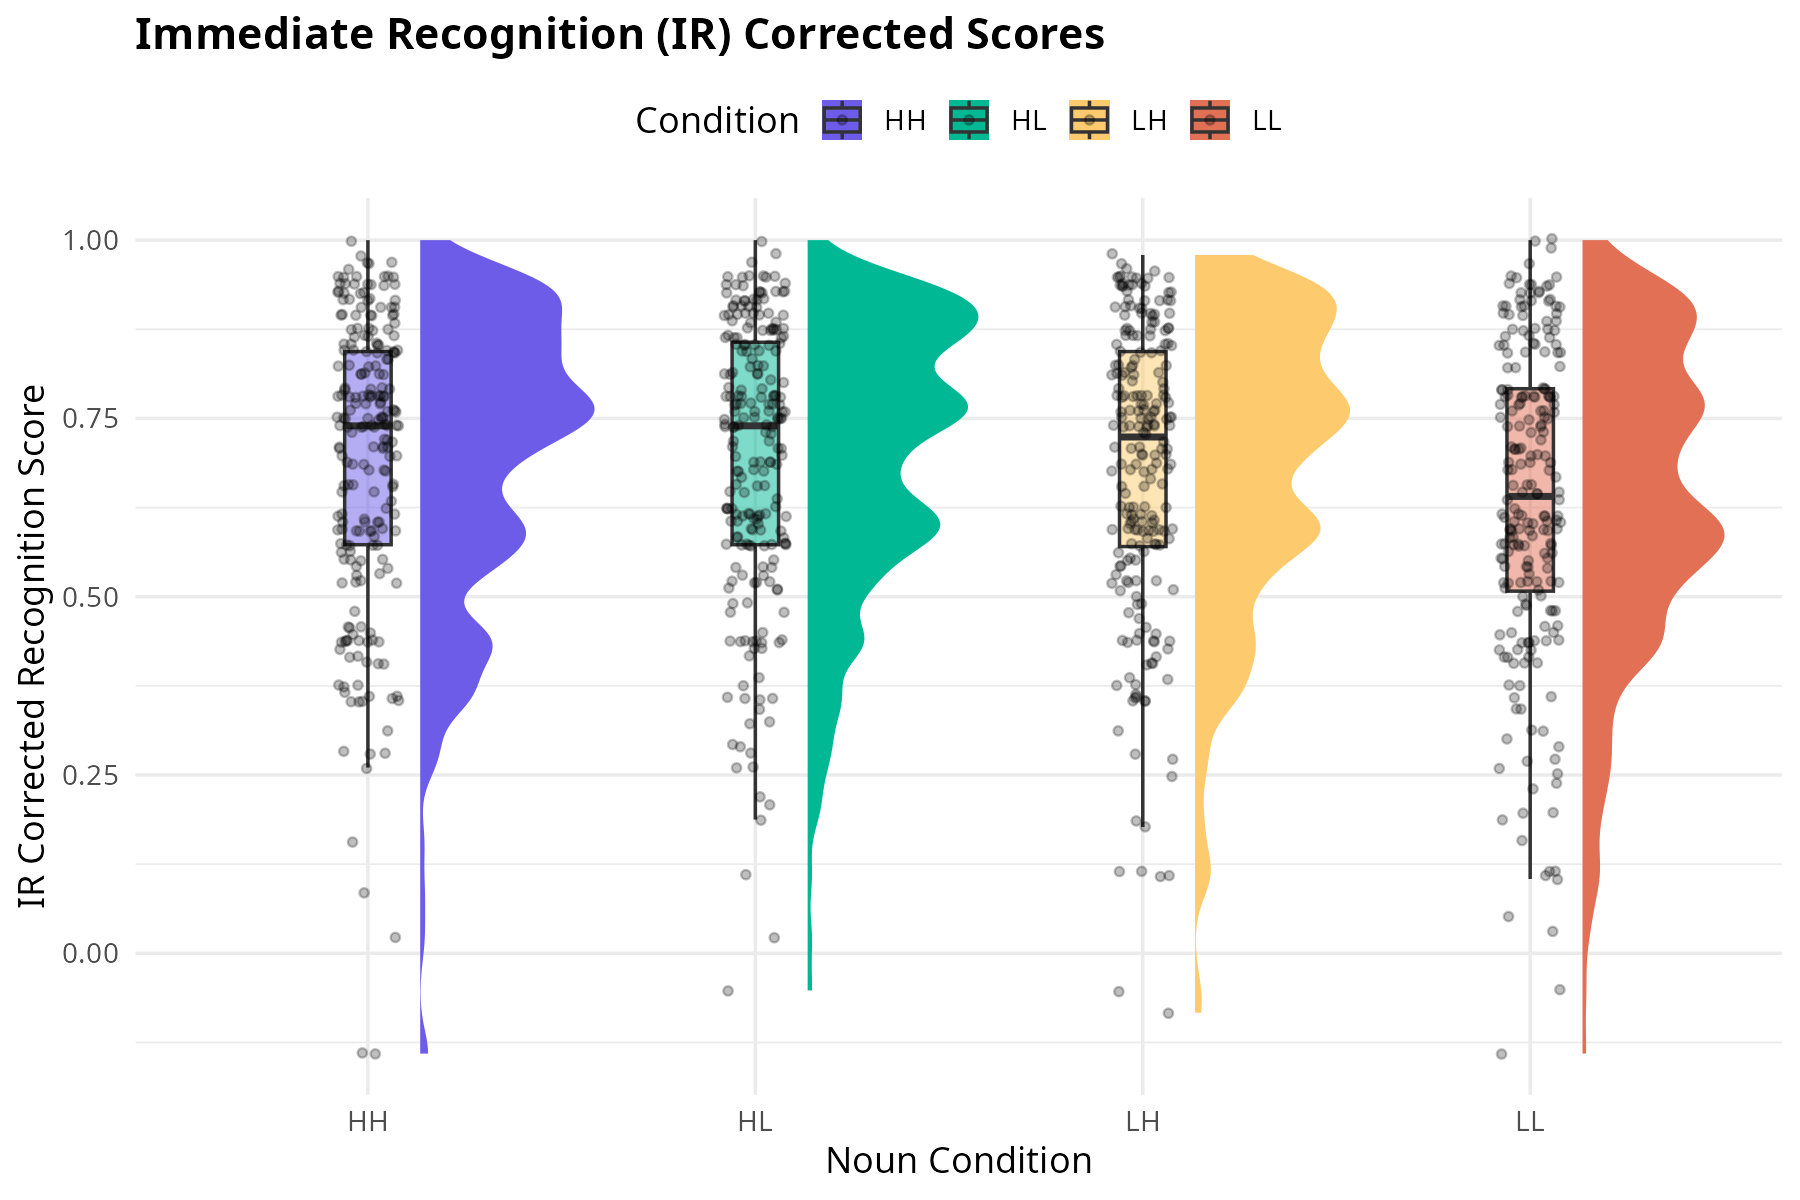
\includegraphics[width=0.90\textwidth, height=0.67\textheight, keepaspectratio]{figures/01_ir_by_condition_raincloud.png}
  \end{center}
  \vspace{-0.3em}
  \small Half-violin = KDE density; box = IQR $\pm$ 1.5 IQR; dots = individual participants.\\
  LL clearly lower; all conditions negatively skewed (ceiling effect).
\end{frame}

\begin{frame}{Raincloud Plot — WR Conditional Accuracy}
  \begin{center}
    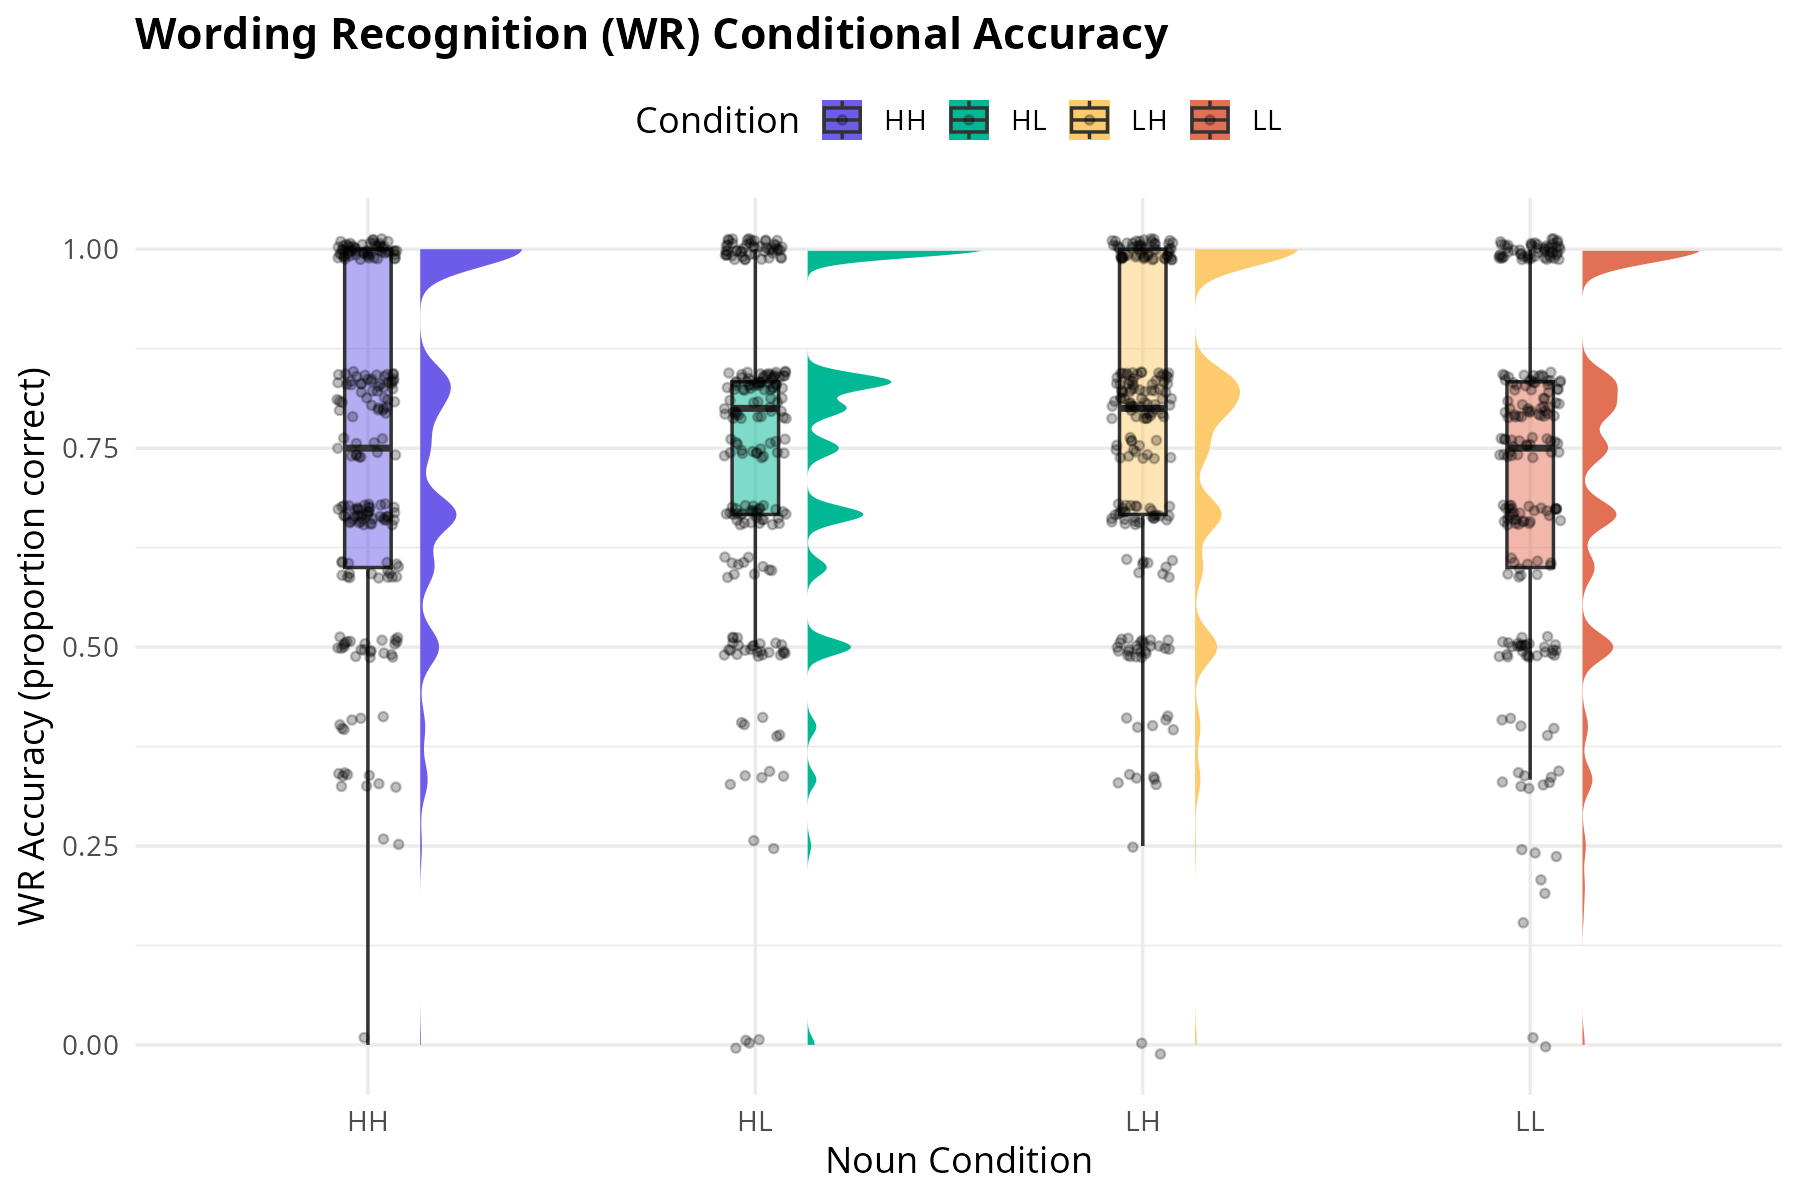
\includegraphics[width=0.90\textwidth, height=0.67\textheight, keepaspectratio]{figures/02_wr_accuracy_raincloud.png}
  \end{center}
  \vspace{-0.3em}
  \small WR accuracy is uniformly high across all conditions.
  No condition stands out as strongly as LL does for IR CR,
  suggesting wording memory is less sensitive to imageability than recognition per se.
\end{frame}

\begin{frame}{Omnibus Test — Kruskal-Wallis}
  \textbf{$H_0$: distributions of metric identical across noun conditions.}
  \vspace{0.6em}
  \begin{center}
  \renewcommand{\arraystretch}{1.25}
  \begin{tabular}{llrrrl}
    \toprule
    \textbf{Metric} & $\chi^2$ & \textit{df} & \pval{} & $\varepsilon^2$ & Result \\
    \midrule
    IR Corrected Recognition (\texttt{ir\_cr})
      & 11.26 & 3 & \sig{.0104} & .013 & \sig{Significant} \\
    WR Accuracy (\texttt{wr\_acc\_score})
      & 2.52  & 3 & \ns{.4714} & .003 & \ns{n.s.} \\
    IR Reaction Time (\texttt{ir\_rt})
      & 5.32  & 3 & \ns{.1495} & .006 & \ns{n.s.}  \\
    \bottomrule
  \end{tabular}
  \end{center}
  \vspace{0.4em}
  \begin{columns}[T]
    \column{0.48\textwidth}
      \begin{exampleblock}{IR CR: significant effect}
        Noun imageability significantly predicts IR CR
        (\kw{3}{11.26}{.010}).\\
        Effect size $\varepsilon^2 = 0.013$ = \textit{small}.
      \end{exampleblock}
    \column{0.48\textwidth}
      \begin{block}{WR accuracy and RT: no effect}
        Neither WR accuracy nor IR RT differed
        significantly across conditions.
      \end{block}
  \end{columns}
\end{frame}

\begin{frame}{Post-hoc Tests — IR Corrected Recognition}
  Pairwise Wilcoxon rank-sum tests with \textbf{Holm correction}
  (only run because KW omnibus was significant) .
  \vspace{0.6em}
  \begin{center}
  \renewcommand{\arraystretch}{1.3}
  \begin{tabular}{lcc}
    \toprule
    \textbf{Pair} & \textbf{Holm-adjusted \pval{}} & \textbf{Verdict} \\
    \midrule
    HH vs HL & 1.000 & \ns{n.s.} \\
    HH vs LH & 1.000 & \ns{n.s.} \\
    HH vs LL & \sig{0.024} & \sig{$p < .05$} \\
    HL vs LH & 1.000 & \ns{n.s.} \\
    HL vs LL & \sig{0.024} & \sig{$p < .05$} \\
    LH vs LL & 0.077 & \ns{marginal} \\
    \bottomrule
  \end{tabular}
  \end{center}
  \vspace{0.4em}
  \begin{alertblock}{Interpretation}
    \textbf{LL (Low-Low imageability) is the outlier}: it scores significantly lower than both HH and HL.
    High imageability in at least one argument position (HH, HL, LH) is sufficient to maintain recognition performance.
    LH vs LL is marginal ($p = .077$), suggesting the \emph{subject} noun imageability may carry slightly more weight.
  \end{alertblock}
\end{frame}

\begin{frame}{Scheirer-Ray-Hare — Noun Condition $\times$ Voice}
  \textbf{Non-parametric 2-factor interaction test} (equivalent of a
  non-parametric two-way ANOVA on ranks).
  \vspace{0.5em}
  \begin{columns}[T]
    \column{0.50\textwidth}
      \begin{block}{DV: IR Corrected Recognition}
        \small
        \renewcommand{\arraystretch}{1.2}
        \begin{tabular}{lrrl}
          \toprule
          Source & $H$ & \pval{} & \\
          \midrule
          Noun condition & 11.26 & \sig{.010} & \sig{*} \\
          Voice          &  0.76 & .384 & \ns{n.s.} \\
          Interaction    &  0.22 & .975 & \ns{n.s.}  \\
          \bottomrule
        \end{tabular}
        \vspace{4pt}
        Noun condition drives the effect;\\
        voice adds nothing; no interaction.
      \end{block}

    \column{0.46\textwidth}
      \begin{block}{DV: WR Accuracy Score}
        \small
        \renewcommand{\arraystretch}{1.2}
        \begin{tabular}{lrrl}
          \toprule
          Source & $H$ & \pval{} & \\
          \midrule
          Noun condition &  2.51 & .473 & \ns{n.s.} \\
          Voice          &  1.19 & .276 & \ns{n.s.} \\
          Interaction    &  4.30 & .231 & \ns{n.s.}  \\
          \bottomrule
        \end{tabular}
        \vspace{4pt}
        Neither main effect nor\\
        interaction reaches significance.
      \end{block}
  \end{columns}
  \vspace{0.4em}
  \small H4 (Voice $\times$ Imageability interaction) is \textbf{not supported}.
\end{frame}

% ============================================================
\section{Diagnostic Plots}
% ============================================================

\begin{frame}{Q-Q Plots — IR Reaction Times}
  \begin{center}
    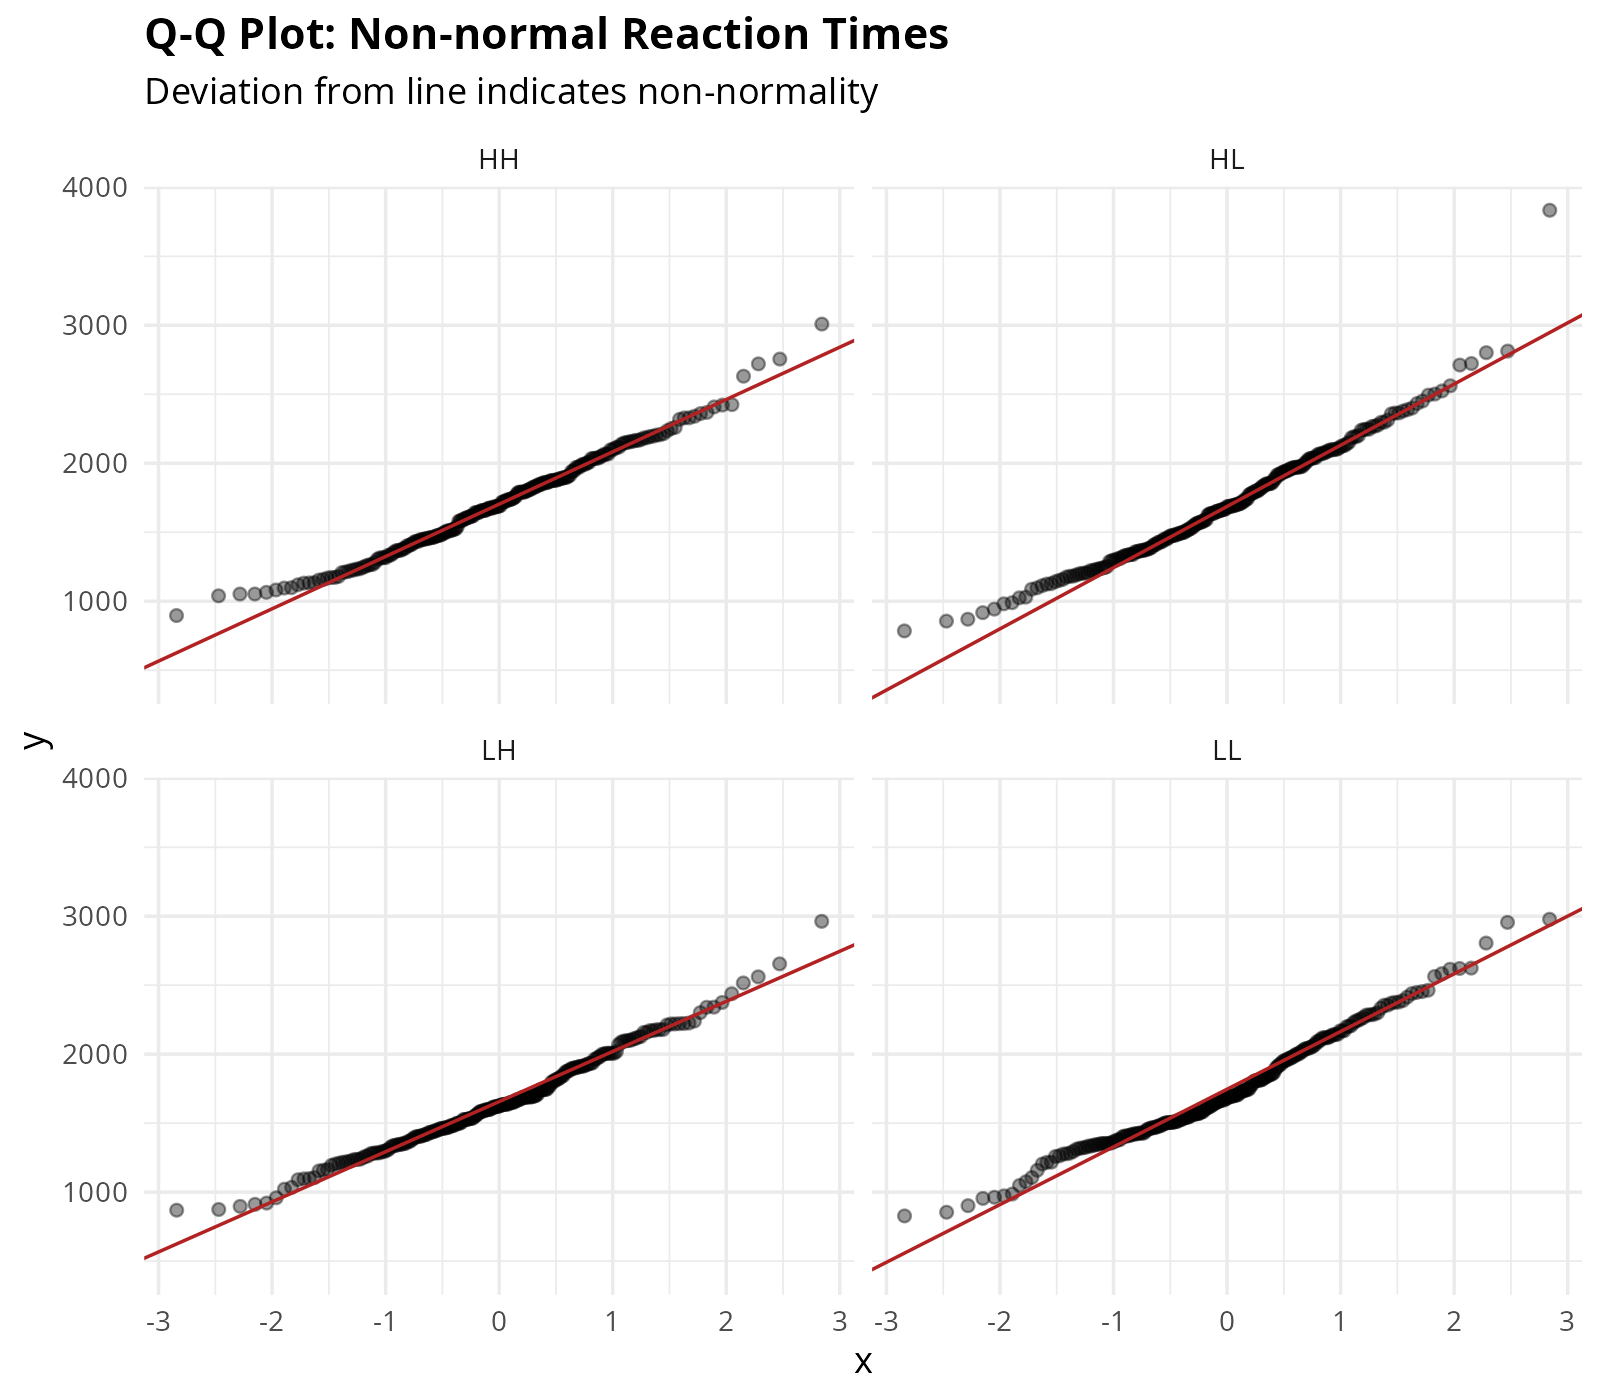
\includegraphics[width=0.88\textwidth, height=0.70\textheight, keepaspectratio]{figures/07_qq_ir_rt.png}
  \end{center}
  \vspace{-0.3em}
  \small Upper quantiles systematically exceed the theoretical normal line
  (right-skew in RT, consistent with log-normal RT distributions) .
  This independently validates the choice of non-parametric methods.
\end{frame}

% ============================================================
\section{Summary \& Discussion}
% ============================================================

\begin{frame}{Summary of Findings}
  \begin{columns}[T]
    \column{0.48\textwidth}
      \textbf{Supported Hypotheses}
      \begin{itemize}
        \item[\checkmark] \textbf{H1} — IR CR is significantly affected by noun imageability (\kw{3}{11.26}{.010}).
        \item[\checkmark] LL is the driver: both HH and HL outperform LL ($p_\text{adj} = .024$).
      \end{itemize}
      \vspace{0.5em}
      \textbf{Unsupported Hypotheses}
      \begin{itemize}
        \item[$\times$] \textbf{H2} — WR accuracy does not differ across conditions ($p = .471$).
        \item[$\times$] \textbf{H3} — IR RT does not differ across conditions ($p = .150$).
        \item[$\times$] \textbf{H4} — No Voice $\times$ Imageability interaction (SRH: $p = .975$).
      \end{itemize}

    \column{0.48\textwidth}
      \begin{exampleblock}{Key Numbers to Remember}
        \footnotesize
        \renewcommand{\arraystretch}{1.2}
        \begin{tabular}{lr}
          \toprule
          Metric & Value \\
          \midrule
          Participants (final) & 112  \\
          Target observations  & 896  \\
          Mean IR FA Rate      & 0.160  \\
          Mean IR CR (HH)      & 0.689  \\
          Mean IR CR (LL)      & 0.632  \\
          Mean WR Accuracy     & 0.747 \\
          KW $\chi^2$ (ir\_cr) & 11.26  \\
          Post-hoc: LL vs HH   & $p = .024$  \\
          \bottomrule
        \end{tabular}
      \end{exampleblock}
  \end{columns}
\end{frame}

\begin{frame}{Discussion}
  \begin{block}{Interpretation of IR Effect}
    The significant effect of noun imageability on IR CR aligns with dual-coding and reconstructive theories. High-imageability words form stronger spatial images, aiding the reconstructive memory trace. The observed threshold effect—where the low-low (LL) condition is the sole outlier—suggests that having at least one highly salient noun is sufficient to anchor the sentence's semantic representation in memory.
  \end{block}
  \vspace{0.4em}
  \begin{block}{Why WR accuracy is unaffected}
    WR accuracy captures form-level memory, which relies on different mechanisms than meaning recognition. Because syntactic structures (like voice) are typically reconstructed rather than stored as independent trace elements, increased imageability strengthens the semantic core without disproportionately enhancing memory for exact wording[cite: 1515, 1926].
  \end{block}
\end{frame}

\begin{frame}{Limitations \& Future Directions}
  \begin{columns}[T]
    \column{0.48\textwidth}
      \textbf{Limitations}
      \begin{itemize}
        \item The final sample of 112 participants falls short of the a-priori power analysis target of 334 required to adequately test our hypotheses[cite: 2176, 1220].
        \item Small effect size ($\varepsilon^2 = 0.013$) limits generalisability.
        \item Drop-out of 2 participants (1.8\%) might introduce minor selection bias.
        \item WR ceiling effect limits power to detect fine imageability differences.
      \end{itemize}

    \column{0.48\textwidth}
      \textbf{Future Directions}
      \begin{itemize}
        \item Increase sample size to match the $N = 334$ recommendation for improved reliability.
        \item Separate subject- and object-noun imageability as independent factors to test asymmetric effects.
        \item Include concreteness as a distinct predictor (separate from imageability).
        \item Add a delayed recognition session ($+24$h) to test whether the imageability effect strengthens over time.
      \end{itemize}
  \end{columns}
\end{frame}

% ── Final slide ──────────────────────────────────────────────
\begin{frame}{}
  \begin{center}
    \vspace{1.5cm}
    {\Huge \textbf{Thank you}}\\[1em]
    {\large Questions?}\\[2em]
    \hrule
  \end{center}
\end{frame}

\end{document}